\documentclass[10pt,twocolumn,letterpaper]{article}

% ---------------------------------------------------------------
% Include basic CVPR package in rebuttal mode

\usepackage[rebuttal]{cvpr}

% ---------------------------------------------------------------
% Other packages

% Commonly used abbreviations (\eg, \ie, \etc, \cf, \etal, etc.)
\usepackage{eccvabbrv}

% Include other packages here, before hyperref.
\usepackage{graphicx}
\usepackage{booktabs}

% The "axessiblity" package can be found at: https://ctan.org/pkg/axessibility?lang=en
\usepackage[accsupp]{axessibility}  % Improves PDF readability for those with disabilities.


% ---------------------------------------------------------------
% Hyperref package
% If you comment hyperref and then uncomment it, you should delete
% egpaper.aux before re-running latex.  (Or just hit 'q' on the first latex
% run, let it finish, and you should be clear).

\definecolor{eccvblue}{rgb}{0.12,0.49,0.85}
\usepackage[pagebackref,breaklinks,colorlinks,citecolor=eccvblue]{hyperref}


% ---------------------------------------------------------------
% If you wish to avoid re-using figure, table, and equation numbers from
% the main paper, please uncomment the following and change the numbers
% appropriately.
%\setcounter{figure}{2}
%\setcounter{table}{1}
%\setcounter{equation}{2}

% If you wish to avoid re-using reference numbers from the main paper,
% please uncomment the following and change the counter for `enumiv' to
% the number of references you have in the main paper (here, 6).
%\let\oldthebibliography=\thebibliography
%\let\oldendthebibliography=\endthebibliography
%\renewenvironment{thebibliography}[1]{%
%     \oldthebibliography{#1}%
%     \setcounter{enumiv}{6}%
%}{\oldendthebibliography}


% ---------------------------------------------------------------
% TODO REBUTTAL: Please enter paper ID
\def\paperID{12200} % *** Enter the paper ID here
\def\confName{ECCV}
\def\confYear{2026}

\begin{document}

% ---------------------------------------------------------------
% TODO REBUTTAL: Paper title is not required
%\title{\LaTeX\ Guidelines for Author Response}  % **** Enter the paper title here

\maketitle
\thispagestyle{empty}
\appendix

% Reviewer tag color helper
\newcommand{\rev}[1]{\textcolor{eccvblue}{[#1]}}

% Tighter spacing around figures
\setlength{\textfloatsep}{5pt}
\setlength{\intextsep}{5pt}
\setlength{\floatsep}{5pt}
\setlength{\abovecaptionskip}{2pt}
\setlength{\belowcaptionskip}{0pt}


% ---------------------------------------------------------------
% TODO REBUTTAL: Enter your response below

\noindent We thank the reviewers for their feedback. In the camera-ready we will fix the GIMDiffusion citation ([15]$\to$[11]) and adopt ``multi-chart geometry image'' consistently. \rev{rPcg minor}

\medskip
\noindent\textbf{\rev{rPcg} DMS-based end-to-end differentiability \emph{to mesh} is the key contribution.} Prior GI works (Omages, GIMDiffusion, GarmageNet) are differentiable only up to image-domain pixel losses, since mesh extraction is a non-differentiable post-process and 3D-domain supervision cannot reach the latent. DMS closes this gap, enabling Normal Rendering Loss to be computed in 3D and back-propagated to the VAE encoder/decoder. Tab.~2 isolates the two effects. Replacing occupancy with TSDF alone reduces CD by $60\%$. Adding the Normal Loss (usable only via DMS) further reduces JSD by $43\%$ and lifts NC from $0.92$ to $0.96$. TSDF~+~DMS~+~$\mathcal{L}_\text{Normal}$ is therefore a coupled contribution that enables 3D end-to-end learning, not a sum of standard components.

\noindent\textbf{\rev{hEpV} Isolating the effect of SD~1.5 VAE initialization.} We use the SD~1.5 VAE only to accelerate convergence; trained on in-the-wild RGB, it carries no geometry-specific prior. (i) Tab.~2 \emph{fixes} the VAE init and varies only the representation: Occ$\to$TSDF reduces CD by $60\%$, demonstrating that the representation contributes independently. (ii) We are also running a from-scratch-vs.-SD-pretrained VAE comparison showing the two converge to comparable final performance (the latter only faster), to be included in the supplementary. % TODO: from-scratch vs SD-pretrained VAE convergence/final-performance experiment

\noindent\textbf{\rev{hEpV} Unified evaluation protocol.} hEpV's comment led us to identify a misstatement in Supp.~Sec.~5 (\emph{``all methods evaluated using DMS''}). The actual protocol uses DMS for TSDF and a Differentiable Tessellation, a differentiable implementation of Omages' native triangulation, for occupancy; the main paper Sec.~4.2 (l.~275--277) already states the latter correctly. Our Differentiable Tessellation contains no mesh-quality engineering and is bit-identical to Omages' native triangulation across all evaluated ABO samples (Fig.~\ref{fig:tess}), introducing no structural advantage or disadvantage when applied uniformly to every occupancy-based baseline.

\begin{figure}[!htbp]
  \centering
  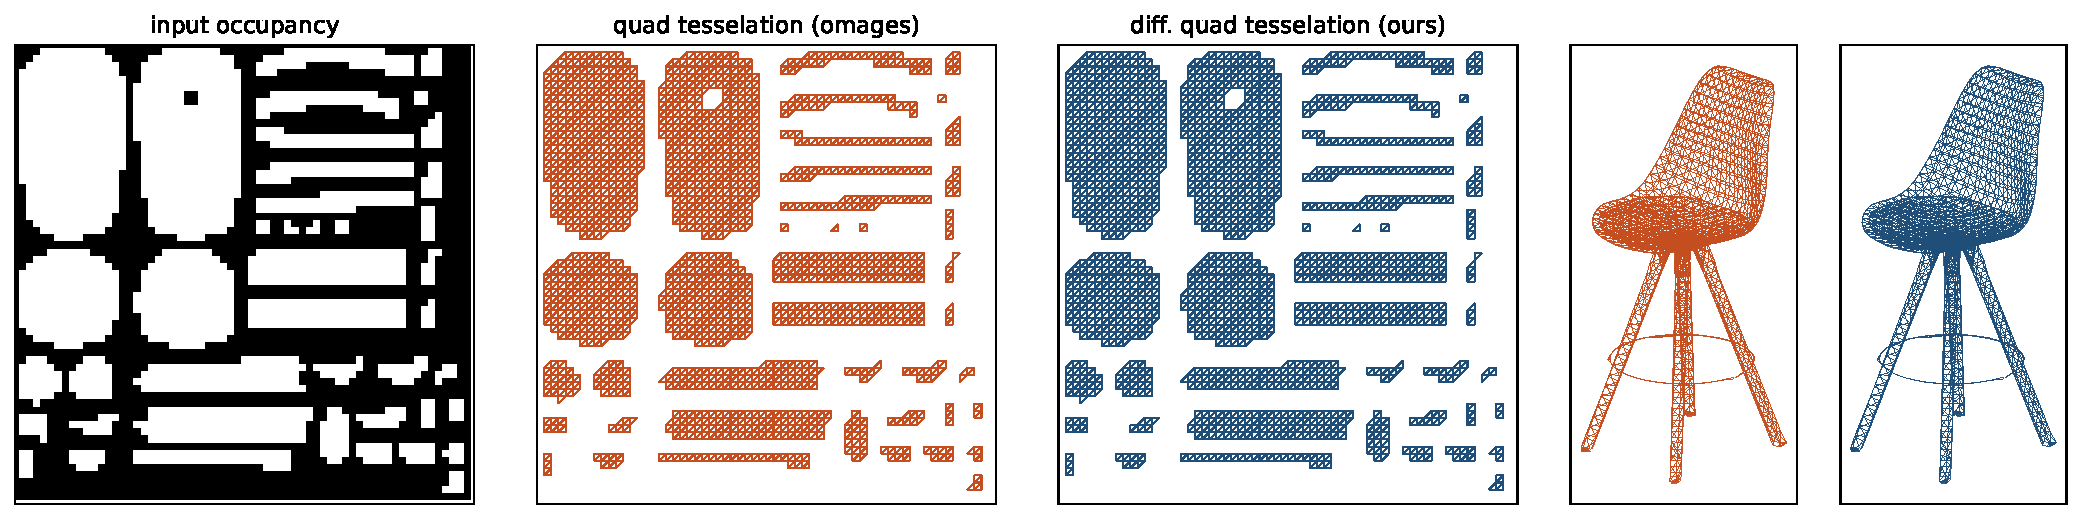
\includegraphics[width=\linewidth]{figures/quad_tessellation}
  \caption{Our Differentiable Tessellation produces output bit-identical to Omages' native occupancy triangulation across all evaluated ABO samples (face count, face set, 3D vertex coordinates).}
  \label{fig:tess}
\end{figure}

\noindent\textbf{\rev{rPcg} Speed vs.\ quality trade-off and structural limits of GarmageNet.} GarmageNet aggressively compresses a dense mesh to 72 dimensions per panel for fast diffusion, but this comes with a quality trade-off. Reconstruction CD on GarmageSet is $4.7\times$ worse (Tab.~1), and image-to-3D BCD is $\sim\!2\times$ worse (Tab.~5). The same is visible in the image-to-3D results of Fig.~6 (main paper): rows~1 and~4 show garment-type changes (skirt$\to$t-shirt; shorts$\to$skirt), other rows show sleeve presence or length mismatches, and row~5 shows a broken form with an anomalous cuff. Its fixed per-panel structure also does not support variable-panel domains such as ABO (l.\,274--275). Our method, without aggressive mesh compression, achieves $\sim\!1$\,s single-GPU latency together with higher quality and generality, resolving this trade-off more effectively.

\noindent\textbf{\rev{rPcg} Why no direct GIMDiffusion comparison.} GIMDiffusion's code, weights, and preprocessed dataset are all unreleased, preventing same-condition reproduction. Nevertheless, its geometry pipeline (binary-mask GI + SD-initialized VAE + LDM; Collaborative Control is texture-only) is structurally equivalent to our \emph{``Occ w/o $\mathcal{L}_\text{Normal}$''} ablation row. Against this baseline, our method (TSDF~+~$\mathcal{L}_\text{Normal}$) improves CD by $3.3\times$ and JSD by $3.6\times$ (Tab.~2). We will make this relationship explicit in the camera-ready.

\noindent\textbf{\rev{ZMhC, hEpV} Characteristics of multi-chart-GI-based diffusion models.} Our method shares the characteristics of this family. (i) Seams: a structural limitation shared by all baselines; we substantially reduce boundary error in BCD (Tab.~5), and further improvement via alternative representations such as dual contouring is left as future work (Sec.~5). (ii) UV dependency: this imposes a dataset-side constraint, but training on industry-standard UVs yields meshes with clean UVs, directly usable in simulation and texturing pipelines. (iii) Resolution: image-based diffusion can scale freely; per the convergence analysis in Supp.~Sec.~1 we adopt resolution~256 in this paper, with higher resolutions planned for follow-up work.

\noindent\textbf{\rev{hEpV} TSDF is a 2D distance in UV-image space, not 3D (l.\,139--141).} It is the signed Euclidean distance from each pixel to the nearest patch contour (positive inside a chart, negative outside), truncated at 15 pixels on the $1024\!\times\!1024$ grid (Sec.~3.1, Step~4); we will state this more clearly in the main text.

\noindent\textbf{\rev{rPcg} Non-cherry-picked ABO generation.} See Tabs.~1, 4, Fig.~5, and Fig.~\ref{fig:abo} for a latent-interpolation sequence between two unrelated samples.

\begin{figure}[!htbp]
  \centering
  
\includegraphics[width=\linewidth]{figures/abo_interpolation}
  \caption{Non-cherry-picked latent interpolation on ABO between two unrelated samples; plausible furniture geometries appear throughout the path.}
  \label{fig:abo}
\end{figure}

%-------------------------------------------------------------------------
% References

{
    \small
    \bibliographystyle{splncs04}
    \bibliography{main}
}

\end{document}